\documentclass[conference]{IEEEtran}
\usepackage[ruled,vlined]{algorithm2e}
\usepackage{amsmath}
\usepackage[english]{babel} %localisation
\usepackage{caption,subcaption} %supposedly incompatible with Springer and IOP, IEEETran and ACM SIG
\usepackage{cite} %nice citations, e.g. [1--5]
\usepackage{fixltx2e} %fix latex bugs
\usepackage{graphicx}
\PassOptionsToPackage{hyphens}{url}\usepackage{hyperref} %clickable URLS
\usepackage[htt]{hyphenat} %hyphenate \texttt
\usepackage{microtype} %makes text pretty; also condenses
\usepackage{multirow} %multiple rows in tables
\usepackage{siunitx,textcomp} %\SI{value}{unit}, \si{unit}; textcomp for microtype compatibility
%\usepackage [caption=false]{subfig} %if caption/subcaption not available
% \usepackage{tikz,pgfplots} %drawings and plots
\usepackage[siunitx]{circuitikz} %circuit figures
\usepackage[T1]{fontenc} %ensure proper hyphenation and treatment of math in sentences
\usepackage{booktabs}
\bibliographystyle{IEEEtran}

\usepackage{tikz}
\usetikzlibrary{shapes}
\usepackage{verbatim}
\usepackage{listings}
\begin{document}
\lstset{defaultdialect=[x86]{Assembler}}

% paper title
% can use linebreaks \\ within to get better formatting as desired
\title{Hardware Trojan: Observing the Invisible}

% author names and affiliations
% use a multiple column layout for up to three different
% affiliations
\author{\IEEEauthorblockN{Nathanael Weidler, Dallin Marshall, Sam Mitchell }
\IEEEauthorblockA{Deptartment of Electrical and Computer Engineering\\
Utah Stat University\\
Logan, Utah 84322\\
e-mail: NWeidler@gmail.com, geekbott@gmail.com, samuel.alan.mitchell@gmail.com}
}

% make the title area
\maketitle


\begin{abstract}
	A VGA-based hardware trojan is proposed and implemented. The trojan observes and leaks a DES key to offscreen pixels on a VGA connection. Implications of this system are discussed. 
\end{abstract}

\begin{IEEEkeywords}
Hardware trojan, security, encryption. 
\end{IEEEkeywords}

\section{Introduction}
	Due to the decreased production costs, many FPGA design firms rely on third-party Intellectual Property cores. These cores may be infected by a hardware trojan meant to disable the device or leak information. Hardware trojans are a growing risk in digital logic production. 
\subsection{Related works}
	Many different types of trojans have been implemented and classified in various taxonomies based on insertion and activation methods \cite{karri2010trustworthy} or by trojan behavior \cite{wang2008detecting}. 

	Multiple detection schemes have been proposed \cite{wolff2008towards,banga2009novel,jha2008randomization}. The two most common schemes are input-based, which uses brute force or other methods to trigger the trojan, and power analysis, which attempts to model and observe the trojan itself. 


\subsection{Structure of paper}
	The organization is as follows: in Section \ref{sec::des_impl}, the development of the PUF is presented.  
	% In Section \ref{sec::expr} the experimental test setup for the capturing of the challenge response pairs is described. 
	Section \ref{sec::analysis} contains the description of the data analysis required to obtain the key. Experimental verification is found in Section \ref{sec:res}. Conclusions are detailed in Section \ref{sec::conclusion}. 


\section{Design} \label{sec::des_impl}
	The proposed hardware trojan attacks a DES encryption algorithm by leaking the key to a VGA monitor. The exploit would be perpetrated by one of the designers at the gate level. In order to avoid detection, the trojan is triggered externally by an input sequence. 

	The trojan is classified into the taxonomy proposed by Karri et al \cite{karri2010trustworthy} in Table \ref{tab:class}. The function of the trojan is better described using the classification proposed by Wang et al \cite{wang2008detecting}. Wang's taxonomy provides a structure for the following sections. 

	% Table generated by Excel2LaTeX from sheet 'Sheet1'
	\begin{table}[htbp]
	  \centering
	  \caption{The proposed hardware trojan is classified according to Karri's taxonomy \cite{karri2010trustworthy}.}
	    \begin{tabular}{ll}
	    \toprule
	    Insertion  & Design, maybe testing \\
	    Abstraction & Gate level \\
	    Activation & External through input sequence \\
	    Effects    & Leak information \\
	    Location   & I/O \\
	    \bottomrule
	    \end{tabular}%
	  \label{tab:class}%
	\end{table}%

	\subsection{Physical characteristics and power}
	The DES implementation obtained for this project was implemented in VHDL \cite{McQueen2003}, with the FPGA driver written by Nathanael Weidler. A size comparison of the original application to the compromised application is found in Table \ref{tab:size}. Our implementation results in a 15\% size increase, but the trigger itself has only a 2\% footprint.

	The small trigger makes it unlikely that the trojan would be detected by a simple power analysis. \cite{jha2008randomization} shows that it is possible to detect. Because the trojan was inserted by a designer, there would be no valid power analysis to compare the clean and infected devices. 
	
	For the sake of this paper the trojan and trigger were removed and then added back into the design incrementally and the Xilinx Xpower Analyzer was used to view the power usage.  For the baseline design, the maximum 170.78 mW.  The trigger added 0.08 mW of power brining the total up to 170.86 mW.  This is only a 0.047\% increase of power caused by the trigger.  Once the trigger has activated the trojan, the maximum power is 172.38 mW.  This is an increase of 1.6 mW over the baseline power or a 0.94\% increase.  This was believed to be very good, especially considering the fact that the trigger increased the power by such a small fraction of a percent that it would likely be lost in the noise unless very advanced techniques were used to detect it.

	% Table generated by Excel2LaTeX from sheet 'Sheet1'
\begin{table}[htbp]
  \centering
  \caption{DES + FPGA application before and after trojan insertion. The percentage is compared to the size of the baseline application. }
    \begin{tabular}{rrrrr}
    \toprule
               & Baseline   & Trigger    & Trojan     & Final  \\
    \midrule
    Flip Flops & 487        & 4          & 80         & 571 \\
    Percent of baseline & 100\%      & 1\%        & 16\%       & 117\% \\
    \midrule
    4-input Look-Up Tables & 883        & 22         & 101        & 1006 \\
    Percent of baseline & 100\%      & 2\%        & 11\%       & 114\% \\
    \midrule
    Total logic elements & 1370       & 26         & 181        & 1577 \\
    Percent of baseline & 100\%      & 2\%        & 13\%       & \textbf{115\%} \\
    \bottomrule
    \end{tabular}%
  \label{tab:size}%
\end{table}%


	This trojan is designed specifically for this DES implementation, but the VGA interaction will work with any design that adheres to the VGA system. This makes the trojan an effective method to leak data through a computer monitor. 

	The insertion model a design team member to insert the gates.  Due to the versatility of the trojan, the system could be inserted during the fabrication and assembly stages. The wiring would be altered to allow additional logic in the fabrication process, followed by adding additional logic during assembly. 

	% Triggering sequence
	\subsection{Trojan activation}
	The trojan utilizes a six-stage trigger activated by a sequence of plaintexts. The last four bits of each plaintext allow the user into the next stage of the trigger. By requiring this specific sequence, the probability of an accidental trigger is $1/2^{24}$. Most testing procedures systematically step through test candidates (1, 2, 3, etc.). Following this method, the trojan would never be triggered. 

	One focus of this trojan is to leak the desired data (key) in a method uncorrelated with the key. There is no reason to perform a one-time pad or other encryption method because the DES permutations obfuscate the key throughout the encryption process. When triggered, the trojan captures the 48-bit outputs of the expansion permutation and round key xor at round 9. See Figure \ref{fig:des}. These values are printed directly to the screen in the method described in Section \ref{s:leak}. The key extraction method is detailed in Section \ref{sec::analysis}. 


	% Exploit leakage. 
	\subsection{Leakage method}\label{s:leak}
	Our attack focuses on a VGA driver. The threat model is as follows: the user sends plaintext to the DES circuit on the FPGA. The FPGA displays the plaintext and ciphertext on a screen via a VGA connection. 

	VGA was originally implemented in 1987 on artifacts of a previous generation --- CRT monitors. The edges of the CRT display are inconsistent, so the VGA driver provides pixel padding, referred to as the front and back porch, on each side of the desired display area. The front and back porches are not displayed on the screen. The padding occurs whether a VGA driver is connected to a CRT or an LCD screen. Our proposed hardware trojan takes advantage of the offscreen area by leaking data to the back porch. The attacker extracts the compromised code by shifting the screen until the compromised pixels appear. 


		\begin{figure}[htbp]
		\centering
		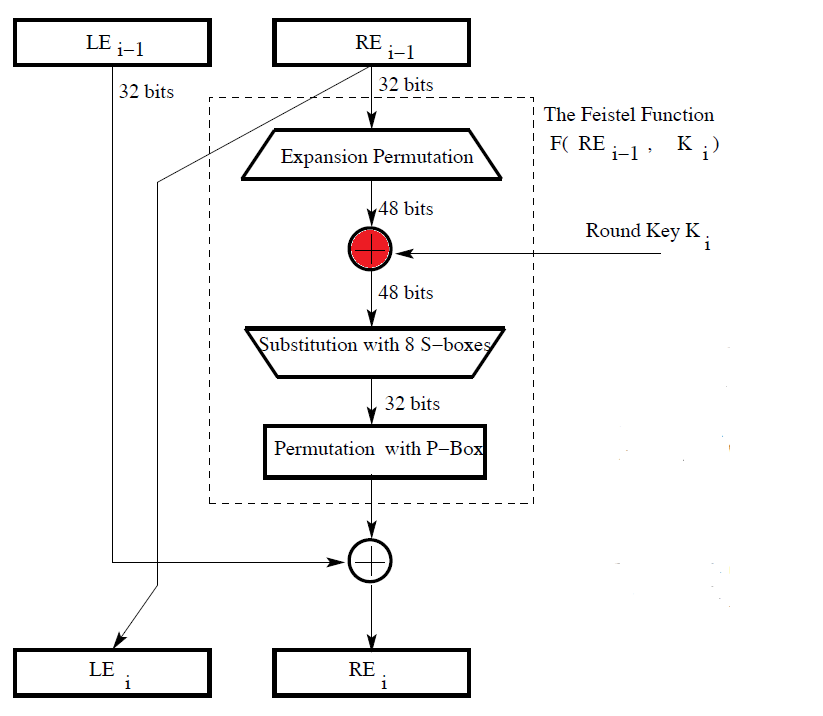
\includegraphics[scale=.4]{des}
		\caption{The trojan leaks the input (expansion permutation) and output of the xor highlighted in red. This leaks the information of the round key without displaying the key itself. }\label{fig:des}
		\end{figure}

\section{Data Analysis}\label{sec::analysis} 
	Our trojan leaked the 48-bit input and output to the round key xor (see Figure \ref{fig:des}). A program was developed to perform the following function: 
	\begin{itemize}
		\item Xor the 48-bit strings to obtain the round key.
		\item Reverse the round key permutations, which results in the known positions of 48 bits of the 56-bit sub-key.
		\item Guess the 8 missing bits of the 56-bit sub-key, followed by reversing the \textit{Permuted Choice 1} operation to obtain the final 8 bits of the 64-bit key. 
		\item Determine the key by encrypting the plaintext using the previous result as key, then comparing the result to the ciphertext shown on the VGA screen. 
	\end{itemize}
\section{Results}\label{sec:res}
	The described trojan was implemented on a Spartan-3E family device, and the output of the system is described. The output on the monitor is displayed by coding the pixels to red and green for 1 and 0, respectively. Figure \ref{fig:blank} shows the screen in default configuration after the trojan was triggered. The item would never be noticed by a normal user. The shifted screen reveals the trojan (Figure \ref{fig:scr}), and the output is codified in Figure \ref{fig:bits}. 

	The output (0x6AAB52A57CA18A70B9489B20) was split into two 48-bit streams, which were then xor-ed together to produce the round key of round 9 (0xE0DBEBEDE781). The program in Section \ref{sec::analysis} was used to reassemble and guess the original 64-bit key (0x133457799BBCDFF1). 
		\begin{figure}[htbp]
		\centering
		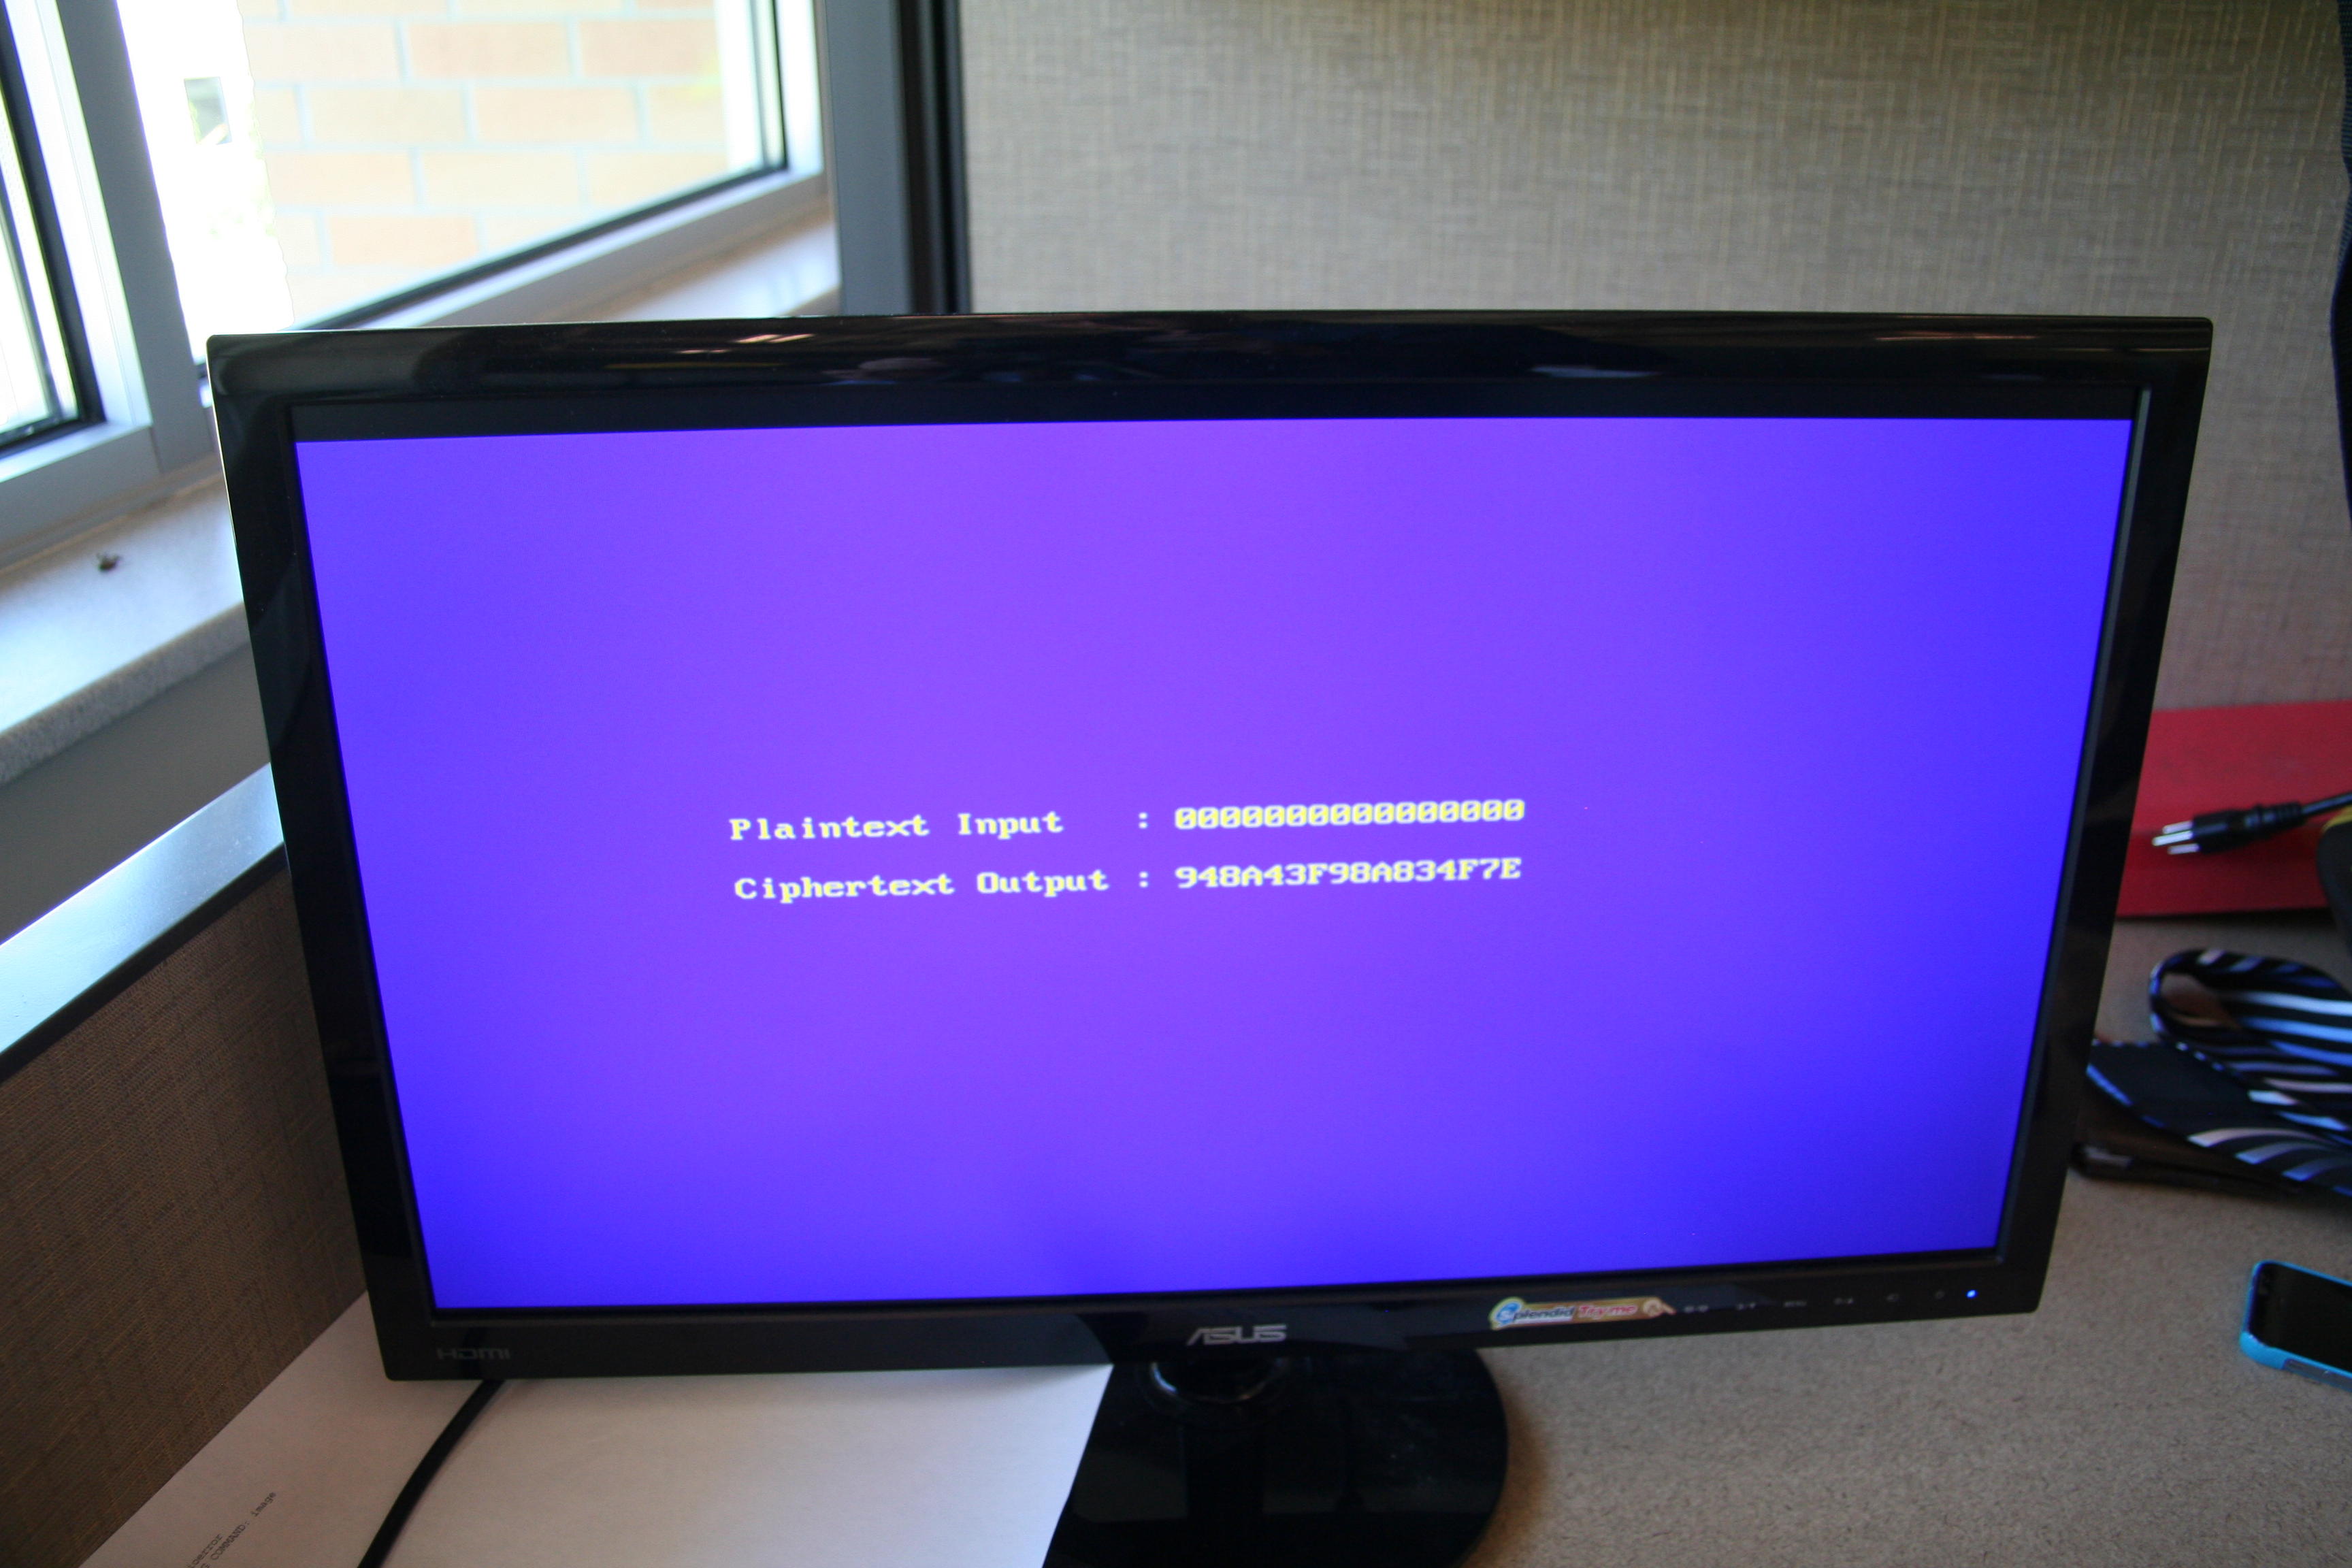
\includegraphics[scale=.05]{monitor}
		\caption{A screen at default configuration. The trojan has been triggered, but it is not visible }\label{fig:blank}
		\end{figure}

		\begin{figure}[htbp]
		\centering
		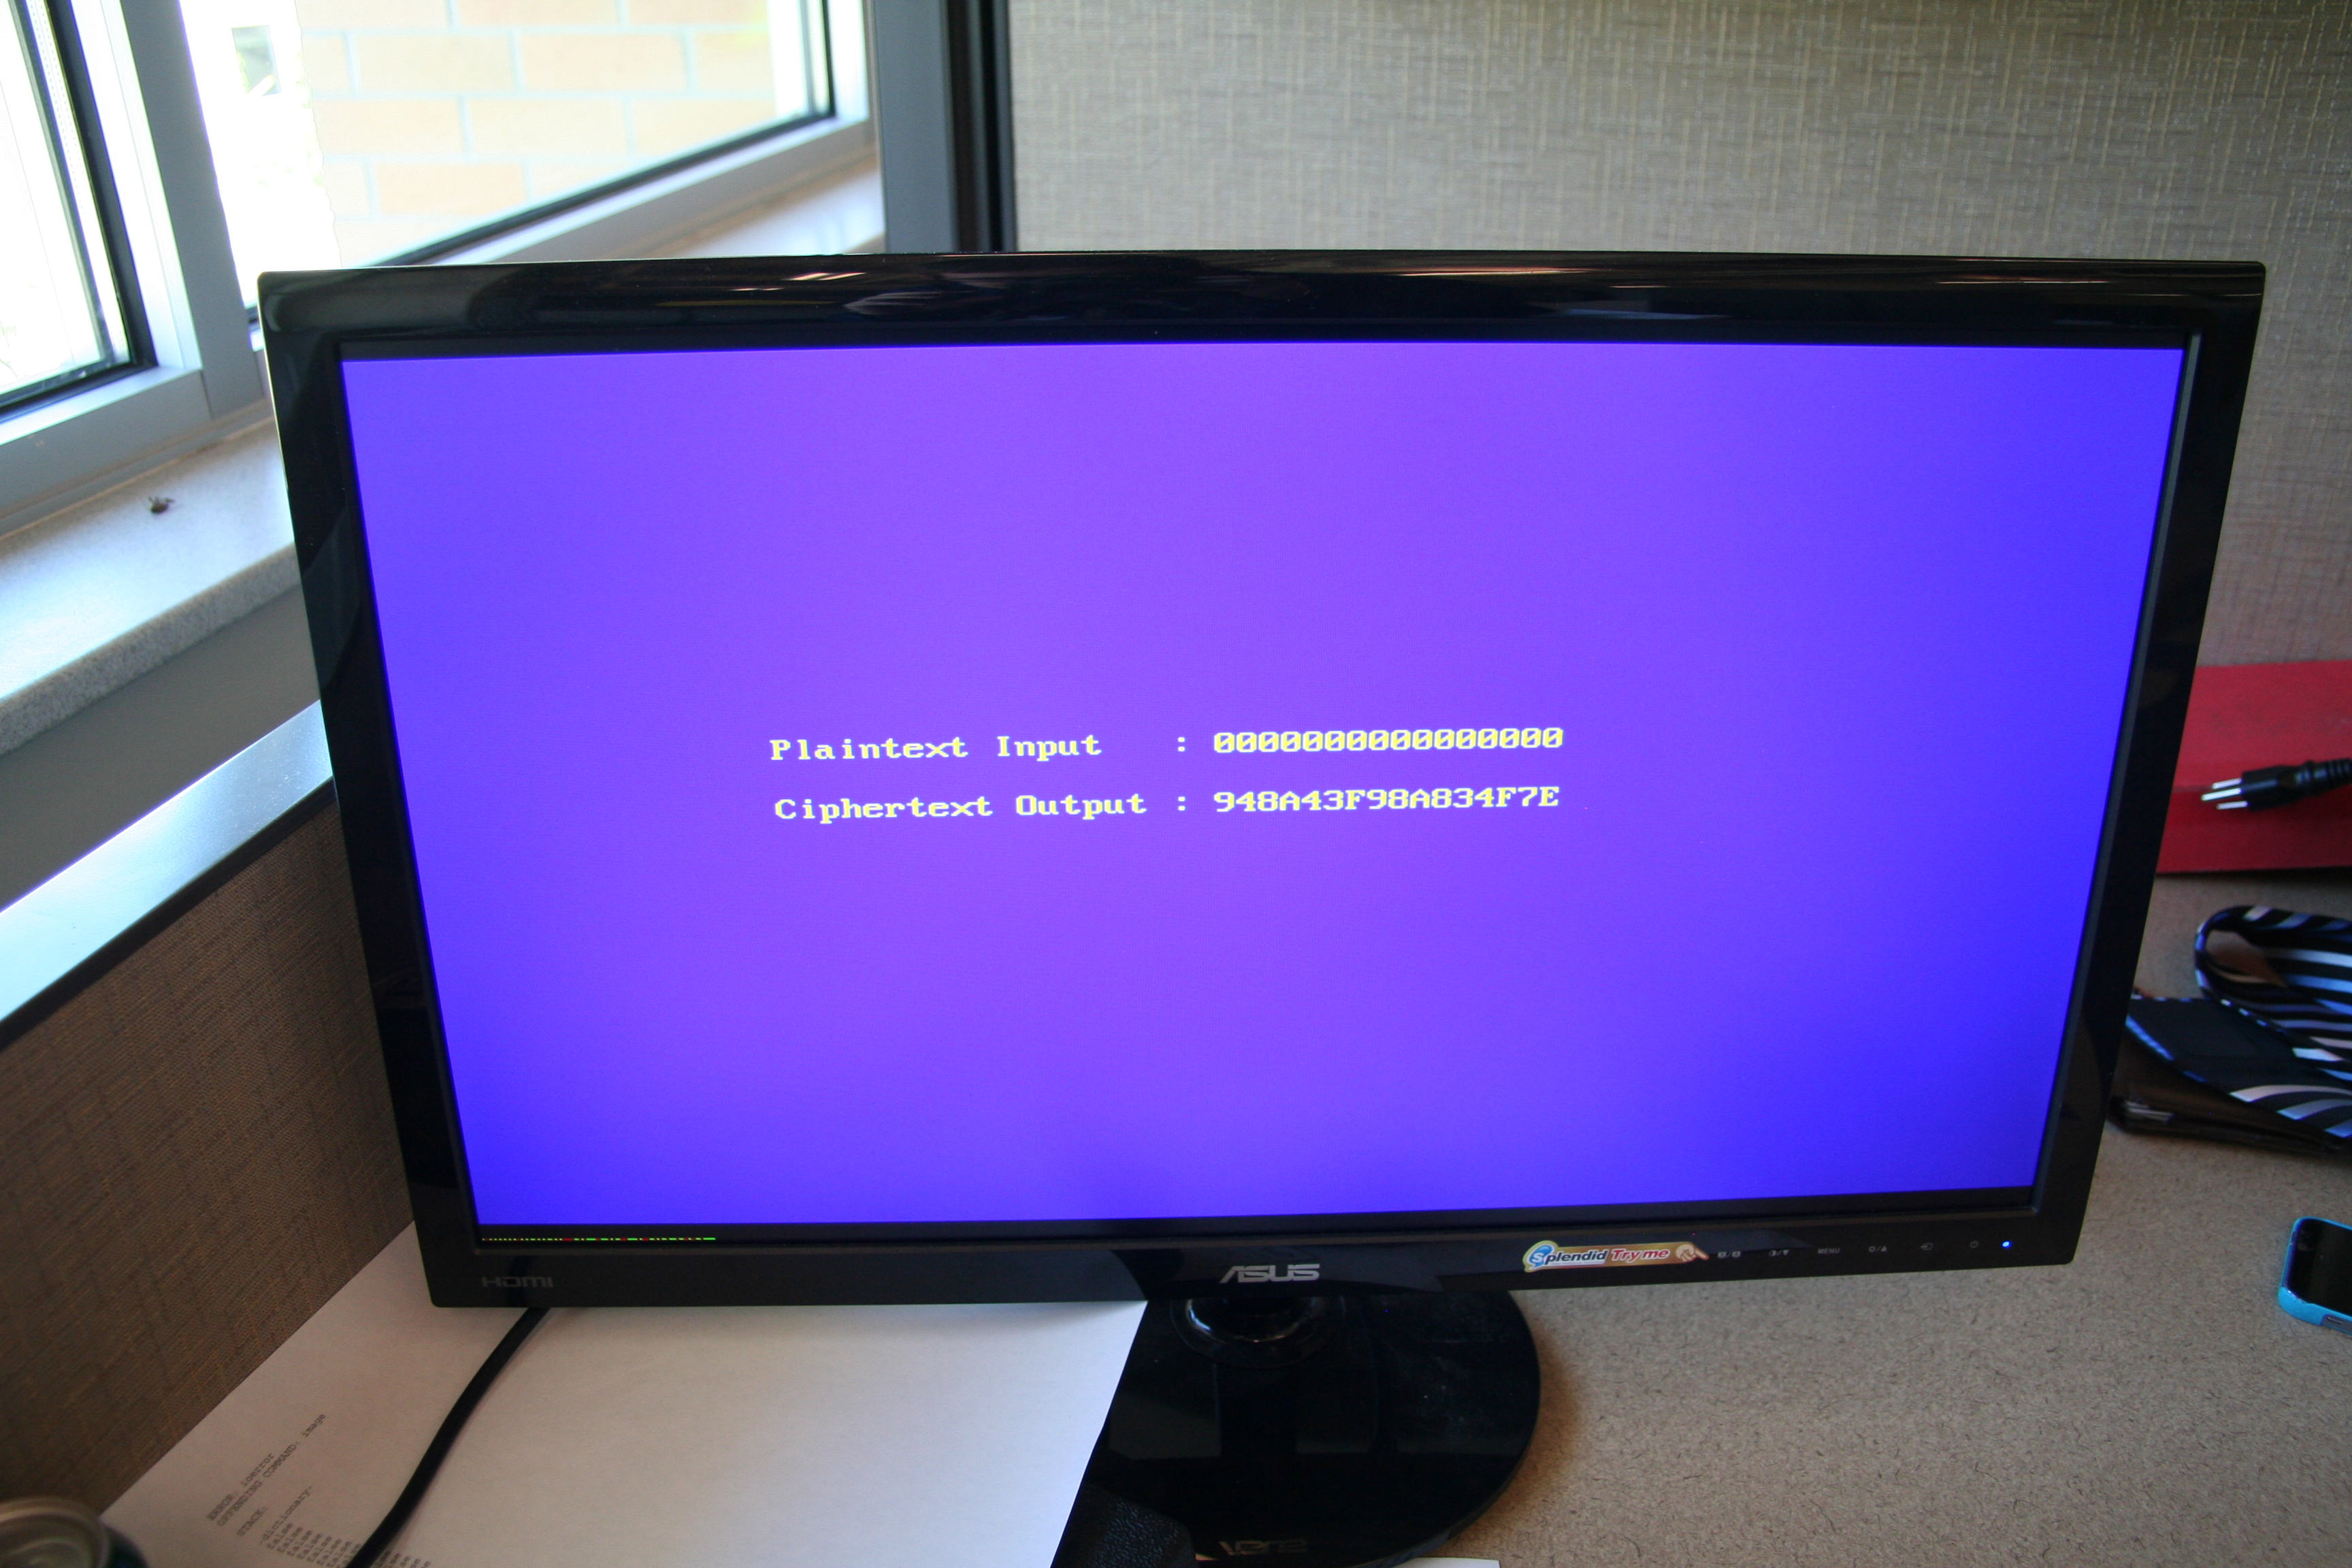
\includegraphics[scale=.05]{screen}
		\caption{A screen that has been shifted to reveal the trojan output. The output is in the bottom left corner of the screen.}\label{fig:scr}
		\end{figure}


		\begin{figure}[htbp]
		\centering
		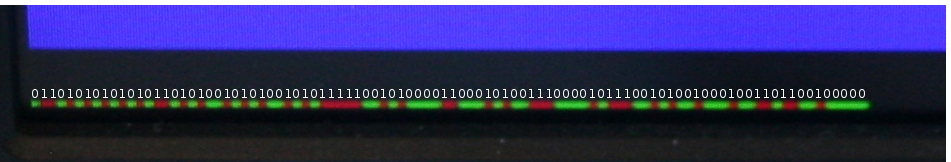
\includegraphics[scale=.2]{bits}
		\caption{The trojan output coded to reveal the bitstream. }\label{fig:bits}
		\end{figure}
\section{Conclusion}\label{sec::conclusion} 
	The proposed hardware trojan is effective because it is hidden by affecting part of an ignored portion of the VGA interface. The obfuscation method removes any correlation between the key and trojan output. Key recovery methods are similar to those used in Side Channel Analysis. Experimental evaluation was performed to verify the functionality of the proposed trojan. 
% \nocite{*}
\bibliography{trojan}
% that's all folks




\end{document}






